\documentclass[11pt,a4paper]{ivoa}
\input tthdefs

\usepackage{array}
\usepackage{tabulary}  % for nicer tables
\usepackage{calc}
\usepackage{placeins}
\setlength\extrarowheight{2pt}

\newcolumntype{L}{>{\centering\arraybackslash}m{3cm}}

\title{Model Instances in Votables}

% see ivoatexDoc for what group names to use here
\ivoagroup{DM}

\newcommand{\TODO}[1]{%
    \noindent%
    \colorbox{todocolor}{%
            \parbox{0.85\linewidth}{\sffamily \textbf{TODO:}\\
            #1}
    }%
    \vspace{2pt}
}

\newcommand{\note}[1]{%
    \noindent%
    \textcolor{darkgrey}{{\sffamily Note:} \emph{#1}}%
}

\newcommand{\comment}[1]{%
    \noindent%
    \textcolor{red}{{\sffamily Comment:} \emph{#1}}%
}

%%%%%%%%%%%%%%%%%%%%%%%%%%%%%%%%%%%%
% XML syntax coloration and formatting
%
\definecolor{todocolor}{rgb}{1,1,0.8}
\definecolor{darkred}{rgb}{0.6,0,0}
\definecolor{rose}{rgb}{1.0,0.88,0.88}
\definecolor{darkgrey}{rgb}{0.35,0.35,0.35}
\definecolor{gray}{rgb}{0.4,0.4,0.4}
\definecolor{darkblue}{rgb}{0.0,0.0,0.6}
\definecolor{maroon}{rgb}{0.5,0,0}
\definecolor{cyan}{rgb}{0.0,0.6,0.6}

\lstset{
  columns=fullflexible,
  showstringspaces=false,
  commentstyle=\color{gray}\upshape
}

\lstdefinelanguage{XML}
{
  morestring=[b]",
  morestring=[s]{>}{<},
  morecomment=[s]{<?}{?>}, 
  morecomment=[s]{<!--}{-->},
  stringstyle=\color{black},
  identifierstyle=\color{darkblue},
  keywordstyle=\color{maroon},
  morekeywords={ref,utype,dmrole, dmtype, value}% list your attributes here
}

\lstdefinestyle{XML}{
    captionpos=b,
    basicstyle=\small\ttfamily
}

%%%%%%%%%%%%%%%%%%%%%%%%%%%
% Document core
%
\author{François Bonnarel}
\author{Gilles Landais}
\author{Laurent Michel}
\author{Jesus Salgado}
\author{Gerard Lemson}

\editor{Laurent Michel}
\editor{Mark Cresitello Dittmar}


% \previousversion[????URL????]{????Concise Document Label????}
\previousversion{This is the first public release}
       

\begin{document}

\begin{abstract}
Vodml-instance-vot (TBD) proposes a syntax to map VOTable data on any model serialized in VO-DML.
Vodml-instance-vot annotations are grouped in a single XML block located in the resource head. 
The annotations operate as a bridge between the data and the model. 
It can denote the way data are connected to each other as well as different tables can be joined together.
It is also able to carry data or meta-data that are missing in the VOTable.
The annotation block is made of bricks that facilitate both annotation process and model instance reconstruction. 
it has been designed so as not to alter the original VOTable content, thus limiting its impact on legacy clients.

\end{abstract}


\section*{Acknowledgments}
CDS/TDIG/SourceDM contributors

\section*{Conformance-related definitions}

The words ``MUST'', ``SHALL'', ``SHOULD'', ``MAY'', ``RECOMMENDED'', and
``OPTIONAL'' (in upper or lower case) used in this document are to be
interpreted as described in IETF standard RFC2119 \citep{std:RFC2119}.

The \emph{Virtual Observatory (VO)} is a
general term for a collection of federated resources that can be used
to conduct astronomical research, education, and outreach.
The \href{http://www.ivoa.net}{International
Virtual Observatory Alliance (IVOA)} is a global
collaboration of separately funded projects to develop standards and
infrastructure that enable VO applications.

\pagebreak
\section{Introduction}

<<<<<<< HEAD

The first purpose of a model is to provide, for a particular domain, a formal description of the relevant quantities and of the way they are connected together .
This documentary role facilitates the communication between the stack-holders and thus the design of interoperability protocols. 

At data level, interoperability consists in arranging searched data in a way that a client can understand them without taking care of their origin. 
So that, the same code can process and compare data coming from different sources.  That way to arrange data is given by the model.

This is not done by default with VOtables because VOTables are containers \citep{2019ivoa.spec.1021O}. 
The VOTable schema cannot say how data are mapped on a given model or whether they match any model at all. 
This is not an issue for simple protocol responses (ref) because the VOTable structure is defined by the protocol itself. 
This is however a big issue for VOTables containing native data such as Vizier  or TAP query responses.

The challenge here is to bind native data with a given model in a way that a model aware software can see them as 
model instances while maintaining the possibility to access them in their original forms.

This is partially done with UTypes which may connect FIELDs or PARAMs with model leaves in the case of simple tree-views of the model. 
Unfortunately, there is nos unique  way to build and parse UTypes in the context of complex models. 
This occurs when e.g the same class is used in different location of the model or when the model contains loops. 
It is also not possible to refer data from different tables with  UTypes.

The landscape has dramatically changed in 2016 when VODML \citep{2018ivoa.spec.0910L} became a recommendation. 
VODML is a meta-model that gives a standard way to express VO models and to make them machine-readable.
In VODML, model leaves are no longer identified by a simple string like UTypes do but by a certain role played in a given location in the model hierarchy.
The consequence is that any annotation mechanism based on VODML will preserve the model hierarchy to save the role played by any components. 
In this context, it might be easy to re-construct model instances from the annotations. 

The main concept of this standard is to insert on the  top of a VOTable resource an XML block compliying with the 
model structures and containing references to the actual data.
In such a way that a model-aware client only has to make a copy of that structure and to resolve the references  
to build an instance. More generic model-unaware clients can just ignore the mapping block. 
=======
The first purpose of a model is to provide,  for a particular domain, a formal description of the relevant quantities and of the way they are connected together .
This documentary role facilitates the communication between the stack-holders and thus the design of interoperability protocols. 

At data level, interoperability consists in arranging searched data in a way that a client can understand them without taking care of their origin. So that, the same code
 can process and compare data coming from different sources.  That way to arrange data is given by the model.

This is not done by default with VOtables because VOTables are containers \citep{2019ivoa.spec.1021O}. The VOTable schema cannot say how data are mapped on a given model 
or whether they match any model at all. This is not an issue for simple protocol responses (ref) because the VOTable structure is defined by the protocol itself. This is 
however a big issue for VOTables containing native data such as Vizier  or TAP query responses.

The challenge here is to bind native data with a given model in a way that a model aware software can see them as model instances while maintaining the possibility to acc
ess them in their original forms.

This is partially done with UTypes which may connect FIELDs or PARAMs with model leaves in the case of simple tree-views of the model. Unfortunately, there is nos unique 
 way to build and parse UTypes in the context of complex models. This occurs when e.g the same class is used in different location of the model or when the model contains
 loops. It is also not possible to refer data from different tables with  UTypes.

The landscape has dramatically changed in 2016 when VODML \citep{2018ivoa.spec.0910L} became a recommendation. VODML is a meta-model that gives a standard way to express 
VO models and to make them machine-readable.
In VODML, model leaves are no longer identified by a simple string like UTypes do but by a certain role played in a given location in the model hierarchy.
The consequence is that any annotation mechanism based on VODML will preserve the model hierarchy to save the role played by any components. In this context, it might be 
easy to re-construct model instances from the annotations. 

The main concept of this standard is to insert on the  top of a VOTable resource an XML block compliying with the model structures and containing references to the actual
 data.
In such a way that a model-aware client only has to make a copy of that structure and to resolve the references  to build an instance. More generic model-unaware clients 
can just ignore the mapping block. 
>>>>>>> b6eb343039aa5f167c2703386d0d2e207f397612



\subsection{Role within the VO Architecture}

\begin{figure}[h]
\centering

% As of ivoatex 1.2, the architecture diagram is generated by ivoatex in
% SVG; copy ivoatex/archdiag-full.xml to archdiag.xml and throw out
% all lines not relevant to your standard.
% Notes don't generally need this.  If you don't copy archdiag.xml,
% you must remove archdiag.svg from FIGURES in the Makefile.

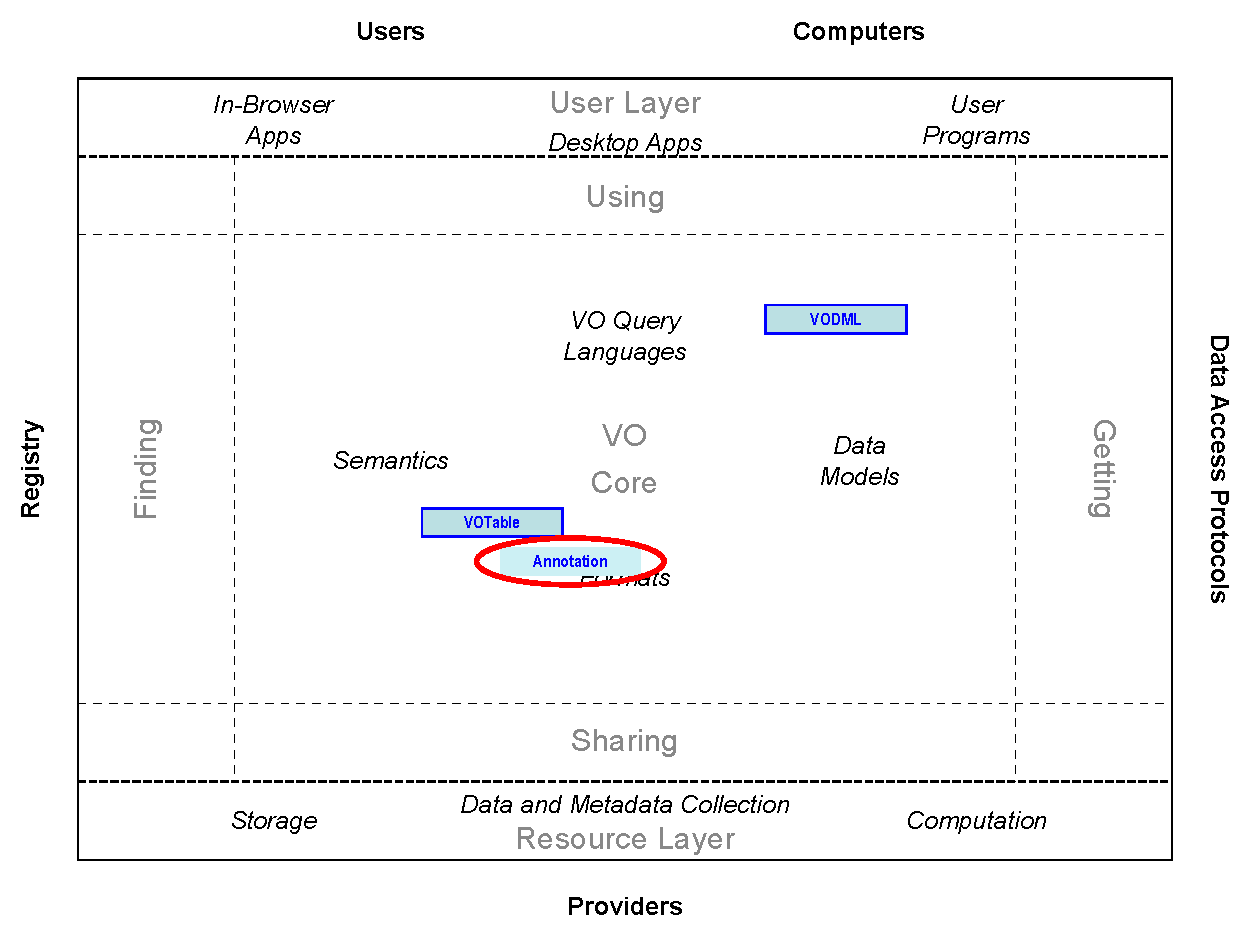
\includegraphics[width=0.9\textwidth]{role_diagram.pdf}
\caption{Architecture diagram for this document}
\label{fig:archdiag}
\end{figure}

Fig.~\ref{fig:archdiag} shows the role this document plays within
the IVOA architecture \citep{2010ivoa.rept.1123A}.


\pagebreak
\section{Use Cases and Requirements}

\subsection{Use Cases}
The meta-data currently supported by the  VOTable standard gives a very good description of the table field content. 
There is however not suitable way to specify the exact role played by a given quantities in a particular context yet.
There is also no way to describe how different quantities or different data tables relate to each others either.
UTypes have been proposed to fill these gaps, but the lack of standard method to build them caused this approach not to be used.
Actually, both role specifications and quantity associations are parts of the modelling effort and our need is a bridge between model leaves and data columns that allows users to get a model view on data tables.
This is essential to get a good  understanding of complex data.

The mapping syntax allows to map data on any model compliant with VODML. 
Annotation blocks denote the model structure and contain references to the appropriate
FIELDs and PARAMs. Model-aware clients can build model instances just by reading the annotation
block and by resolving the references to set the model leaf values. 

Such a mechanism allows the client to get a better understanding of the data complexity.
The annotation block is designed in a way that clients are not forced to choose between a regular data processing and a full object approach.
There are intermediate levels of use that correspond to concrete use cases that are addressed by this standard.



\begin{itemize}
  \item Coordinate or calibration Systems: The recent modelling efforts (Coord and PhotDM) provide a very accurate description of coordinate frames or photometric systems that need to be serialised in VOTables:
  \begin{itemize}
    \item Clients often need to get an accurate representation of the coordinate systems to make the best of many datasets  
    \item Data sets can contain multiple quantities expressed in the same coordinate system (corrected position vs raw position) or 
             quantities of the same nature but expressed in different systems (sky coordinates in IRCS vs Gal). VOTable currently do not support the latest pattern.
  \end{itemize} 
  
  \item Quantities made with multiple components (data columns) that must be gathered by the client to be properly used:
  \begin{itemize}
    \item value-error associations
    \item error quantities split in several columns (covariance matrices). 
    \item quantities with quality flags
    \item positions with proper motions and/or parallax to compute error ellipses or positions at a given epoch
  \end{itemize} 

  \item The above cases relate to the processing of individual datasets; the model annotations become even more important for cases where a good level of interoperability is required to match different datasets. 
           This can be achieved by giving a common data structures for all quantities of interest. This is the purpose of e.g. Measure model that proposes classes for 
           most of the physical quantities and that can be rendered by the mapping syntax. Measure classes are not meant to be used as standalone elements but as parts of host models (e.g. CubeDM, Mango);
           however clients keep free to either process those host models as a whole or to chase individual components.
    \begin{itemize}
      \item Cross matching VOTables having all the same accurate description of e.g. the sky position is easier. 
               This also improves the reliability of the process since the engine does not need to infer information that is not in the FIELD meta-data.
      \item Building SEDs from datasets that have the same accurate photometry representation is straightforward.
   \end{itemize}          

  \item I more advanced cases, we need to be able to extract complete model instances from VOTables.
    \begin{itemize}
      \item Extracting a TimeSeries instances to feed a software built upon classes generated from that model.
      \item Building model instances that can be serialised in another format e.g. json to be share in another context than the VOTable processing e.g. SAMP
   \end{itemize}          
    
\end{itemize} 




\subsection{Requirements}
Model agnostic

not breaking the VOTable schema

Must not impact the legacy clients

Able to reproduce any VODML compliant model

parsable at different levels with regular software


% use XML formatting for listings
\lstset{language=XML}

\pagebreak
\section{Relation to VOTable}

The data model annotation will reside within the scope of a VOTABLE V1.1+

\noindent \textbf{Location}

The mapping block:
\begin{itemize}
\item MUST be contained in a VOTable RESOURCE with \texttt{type="meta"}.
\item which MUST be the first child of a RESOURCE with \texttt{type="results"}.
\item there MUST be no more than one mapping block per 'results' RESOURCE.
\end{itemize}

The scope of the mapping block is the whole content of the 'results' RESOURCE. \newline

\noindent \textbf{Namespace}

The \texttt{dm-mapping} name space isolates VOTable elements from mapping elements, and MUST be defined on the mapping block. \newline

\begin{lstlisting}[frame=single,caption={Mapping block in a VOTable},style=XML,basicstyle=\tiny]
<VOTABLE xmlns="http://www.ivoa.net/xml/VOTable/v1.3" 
         xmlns:xsi="http://www.w3.org/2001/XMLSchema-instance" version="1.3">
  <RESOURCE type="results">
    <RESOURCE type="meta">
      <dm-mapping:VODML xmlns:dm-mapping="http://www.ivoa.net/xml/merged-syntax">
        ...
      </dm-mapping:VODML>
    </RESOURCE>
    <TABLE name="myDataTable">
      ....
    </TABLE>
  </RESOURCE>
</VOTABLE>
\end{lstlisting}


\pagebreak
\section{Syntax}

  \begin{figure}[h]
    \begin{center}
      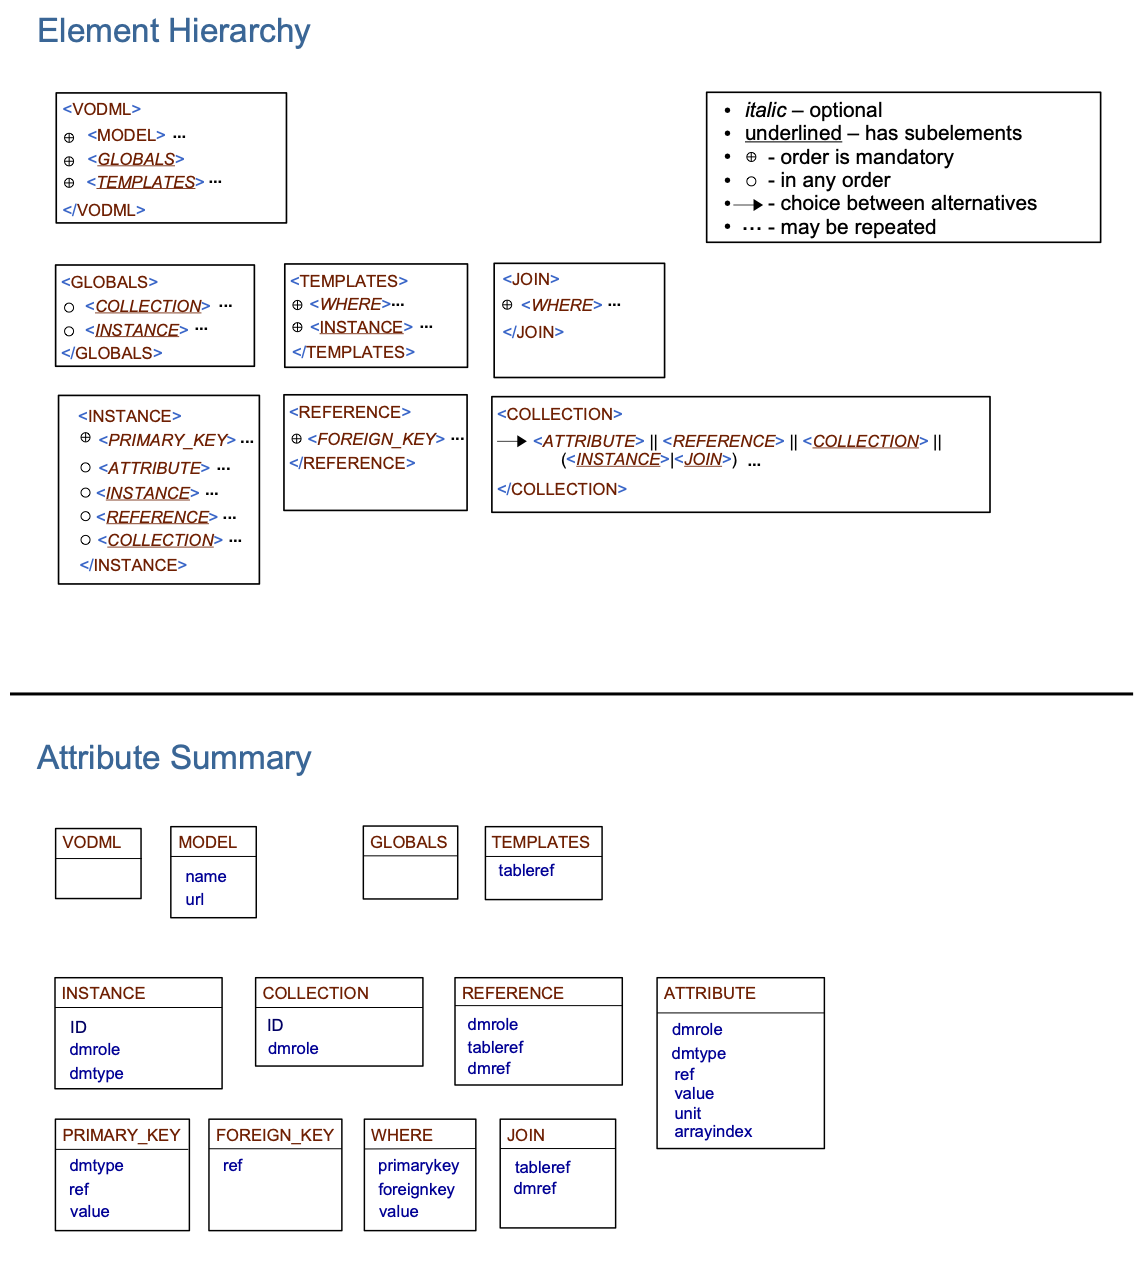
\includegraphics[width=\textwidth]{merged-syntax-summary.png}
      \caption{Annotation Syntax Summary}
      \label{fig:summary}
    \end{center}
  \end{figure}

\pagebreak
\subsection{VODML}
The VODML element is the top level container for the mapping elements for a single VOTable RESOURCE.
When the mapping REPORT is set to KO, the others  VOTable children are optional.

\begin{lstlisting}[frame=single,caption={Example VODML mapping block},style=XML,basicstyle=\tiny]
<dm-mapping:VODML>
  <dm-mapping:REPORT status="OK"/>
  <dm-mapping:MODEL>  ...  </dm-mapping:MODEL>
  <dm-mapping:GLOBALS>  ...  </dm-mapping:GLOBALS>
  <dm-mapping:TEMPLATES>  ...  </dm-mapping:TEMPLATES>
   ...
</dm-mapping:VODML>
\end{lstlisting}

\begin{table}[!htbp]
  \small
  \centering
  \begin{tabulary}{\linewidth}{|c |c |c|}
    \hline 
        \textbf{Element} &
        \textbf{Position} &
        \textbf{Occurs}\\
    \hline
    \hline  
      \texttt{REPORT} &           
      1 &           
      0-1\\
    \hline  
      \texttt{MODEL} &           
      2 &           
      0-*\\
    \hline    
      \texttt{GLOBALS} &           
      3 &           
      0-*\\
    \hline  
      \texttt{TEMPLATES} &           
      4 &           
      0-*\\
    \hline 
  \end{tabulary}
    \caption{Allowed children for \texttt{VODML}} 
    \label{tbl:vodml-children}
\end{table}



\FloatBarrier

\subsection{REPORT}
Services providing annotated responses must use the \texttt{REPORT}  element to tell the client whether the annotation process succeeded or not.

\begin{itemize}
\item \texttt{REPORT} is not mandatory.
\item It must be the first \texttt{VODML} child if present.
\end{itemize}



\begin{lstlisting}[frame=single,caption={Example of a REPORT element},style=XML,basicstyle=\tiny]
<dm-mapping:VODML
	xmlns:dm-mapping="http://www.ivoa.net/xml/merged-syntax">
	
	<dm-mapping:REPORT status="KO">
	    The annotation process failed
	</dm-mapping:REPORT>

	<dm-mapping:MODEL name="model" url="http://aaaaaa" />
	<dm-mapping:MODEL name="model" />
	
</dm-mapping:VODML>
\end{lstlisting}

\begin{table}[!htbp]
  \small
  \centering
  \begin{tabulary}{\linewidth}{|c|J|}       
    \hline 
         \textbf{Attribute} & 
         \textbf {Role}\\
    \hline
    \hline  
         @status  & 
        Status of the annotation process; must be either \texttt{OK} or \texttt{KO} \\
    \hline 
  \end{tabulary}
  \caption{\texttt{REPORT} attributes} 
  \label{tbl:model-att}
\end{table}


\FloatBarrier
 
\subsection{MODEL}
A VOTable can provide serializations for an arbitrary number of data model
types. In order to declare which models are represented in the file, data
providers must declare them through the MODEL elements.
Only models that are used in the file must be declared. A model is
used if at least one element in the mapping block refer to it. In other terms, only models that define vodml-ids used in the
annotation must be declared.

\begin{lstlisting}[frame=single,caption={Example MODEL mapping block},style=XML,basicstyle=\tiny]
<dm-mapping:VODML>
  <dm-mapping:MODEL name="sample-ext"
                     url="https://www.myorg.net/models/SampleExt-v1.0.vo-dml.xml" />
  <dm-mapping:MODEL name="sample" url="https://www.ivoa.net/xml/DNE/Sample-v1.0.vo-dml.xml" />
  <dm-mapping:MODEL name="ivoa"   url="https://www.ivoa.net/xml/VODML/IVOA-v1.vo-dml.xml" />
</dm-mapping:VODML>
\end{lstlisting}

\begin{table}[!htbp]
  \small
  \centering
  \begin{tabulary}{\linewidth}{|c|J|}       
    \hline 
         \textbf{Attribute} & 
         \textbf {Role}\\
    \hline
    \hline  
         @name  & 
         Name of the mapped model as declared in the VODML/XML model serialization.  This attribute MUST not be empty and forms the prefix used in dmrole/dmtype tags of elements from that model.  \\
    \hline 
         @url & 
         URL to the vo-dml serialization of the model. If present, this attribute MUST not be empty.\\
    \hline 
  \end{tabulary}
  \caption{\texttt{MODEL} attributes} 
  \label{tbl:model-att}
\end{table}


\begin{table}[!htbp]
  \small
  \centering
  \begin{tabulary}{\linewidth}{|c |c |J|}
    \hline 
        \textbf{@name} &
        \textbf{@url} &
        \textbf{Pattern}\\
    \hline      \hline  
        MAND &           
        OPT &           
        Unique attribute pattern supported by \texttt{MODEL}\\
    \hline 
  \end{tabulary}
  \caption{Valid attribute patterns for  \texttt{MODEL}} 
  \label{tbl:model-pattern}
\end{table}

\FloatBarrier

\subsection{GLOBALS}
The \texttt{GLOBALS} block holds singular data model instances, and is not associated 
with a VOTable \texttt{TABLE}.

The contained instances have a global scope, and may be
referenced by other instances anywhere in the mapping block.  \texttt{INSTANCE} attributes
within the \texttt{GLOBALS} scope may only refer to VOTable \texttt{PARAMS} or contain
explicit values, they MUST NOT refer to VOTable \texttt{FIELDS}.  Note: This rule is not enforced
via the XSD schema which is restricted to the mapping block only.

Related instances may be grouped within a \texttt{COLLECTION} block to enable selection
via the ORM elements provided in this syntax.  See \texttt{COLLECTION} for more details.

\begin{lstlisting}[frame=single,caption={Example \texttt{GLOBALS} block},style=XML,basicstyle=\tiny]
<dm-mapping:VODML>
  <dm-mapping:MODEL name="sample" url="https://www.ivoa.net/xml/DNE/Sample-v1.0.vo-dml.xml" />
  <dm-mapping:MODEL name="ivoa"   url="https://www.ivoa.net/xml/VODML/IVOA-v1.vo-dml.xml" />
  <dm-mapping:GLOBALS>
    <!-- a collection of coordinate systems -->
    <dm-mapping:COLLECTION dmid="\_CoordinateSystems" >
      <dm-mapping:INSTANCE dmid="\_timesys" dmtype="sample:TimeSys">
         ...
      </dm-mapping:INSTANCE>
      <dm-mapping:INSTANCE dmid="\_spacesys" dmtype="sample:SpaceSys">
         ...
      </dm-mapping:INSTANCE>
    </dm-mapping:COLLECTION>

    <!-- a singular, stand-alone instance -->
    <dm-mapping:INSTANCE dmtype="sample:Thing">
      <dm-mapping:ATTRIBUTE dmrole="sample:Thing.name" dmtype="ivoa:string" value="MyThing"/>
      <dm-mapping:ATTRIBUTE dmrole="sample:Thing.date" dmtype="ivoa:string" ref="\_date"/>
      ...
    </dm-mapping:INSTANCE>
  </dm-mapping:GLOBALS>
</dm-mapping:VODML>
\end{lstlisting}


\begin{table}[!htbp]
  \small
  \centering
  \begin{tabulary}{\linewidth}{|c |c |c|}
    \hline 
        \textbf{Element} &
        \textbf{Position} &
        \textbf{Cardinality}\\
    \hline
    \hline
        \texttt{INSTANCE} &
        Any &
        0-*\\
    \hline
        \texttt{COLLECTION} &
        Any &
        0-*\\
    \hline
  \end{tabulary}
  \caption{Allowed children for \texttt{GLOBALS}} 
  \label{tbl:globals-children}
 \end{table}

\FloatBarrier

\subsection{TEMPLATES}

\begin{table}[!htbp]
\small
\centering
\begin{tabulary}{\linewidth}{|c|J|}       
       \hline 
            \textbf{Attribute} & 
            \textbf {Role}\\
       \hline         \hline  
            @tableref & 
            ID of the mapped table.  \\
        \hline 
     \end{tabulary}
     \caption{\texttt{TEMPLATES} attributes} 
     \label{tbl:templates-att}
 \end{table}

\begin{table}[!htbp]
\small
\centering
\begin{tabulary}{\linewidth}{|c|J|}
    \hline 
        \textbf{@tableref} &
        \textbf{Pattern}\\
    \hline      \hline  
        OPT &           
        If @tableref is not present, \texttt{TEMPLATES} maps the first \texttt{TABLE} of the \texttt{RESOURCE}\\
   \hline 
\end{tabulary}
     \caption{Valid attribute patterns for  \texttt{TEMPLATES}} 
     \label{tbl:templates-pattern}
 \end{table}

\begin{table}[!htbp]
\small
\centering
\begin{tabulary}{\linewidth}{|c |c |c|J|}
    \hline 
        \textbf{Element} &
        \textbf{Position} &
        \textbf{Cardinality} &
        \\
    \hline      \hline  
        \texttt{WHERE}  &        
        1 &           
        0-* &
        The mapping must be applied to the rows matching the \texttt{WHERE} condition only\\
    \hline    
        \texttt{INSTANCE} &           
        2 &           
        0-* &
        Mapped class instances\\
    \hline 
\end{tabulary}
     \caption{Allowed children for \texttt{TEMPLATES}} 
     \label{tbl:templates-chilren}
 \end{table}
\FloatBarrier

\subsection{COLLECTION}
    COLLECTION is a container element.  It is used in different contexts, each allowing a limited subset of elements for its content. 

    \begin{enumerate}
    \item{As child of INSTANCE}
      
      The COLLECTION serves as a container for elements with multiplicity $>$ 1.\\
      Examples of usage in this context would be:
      \begin{itemize}
        \item an array attribute
        \item a reference relation with multiplicity $>$ 1
        \item a composition relation with multiplicity $>$ 1
      \end{itemize}
      
    \item{As child of GLOBALS}
          
      The COLLECTION serves as a proxy for TABLE, grouping common INSTANCES for selection by PRIMARY/FOREIGN\_KEY.
      Examples of usage in this context would be:
      \begin{itemize}
        \item a set of photometry filters, which apply to various rows of a photometric data table, based on the value of the 'band' column.
        \item a set of Dataset metadata instances, which apply to various rows of a photometric data table, based on the value of the 'band' column.
      \end{itemize}
          
    \item{As child of COLLECTION}

          The use-case for this is unclear
        
    \end{enumerate}
   
\begin{lstlisting}[frame=single,caption={Example of COLLECTION child of INSTANCE},style=XML,basicstyle=\tiny]
<dm-mapping:INSTANCE dmtype="model:Thing">
    <dm-mapping:COLLECTION dmrole="model:Thing.elems">
        <dm-mapping:ATTRIBUTE dmtype="model:Foo" value="100" />
        <dm-mapping:ATTRIBUTE dmtype="model:Foo" value="110" />
    </dm-mapping:COLLECTION>
</dm-mapping:INSTANCE>
\end{lstlisting}   

\begin{lstlisting}[frame=single,caption={Example of COLLECTION child of GLOBALS},style=XML,basicstyle=\tiny]
<dm-mapping:GLOBALS>
    <dm-mapping:COLLECTION dmid="_filters" >
        <dm-mapping:INSTANCE dmtype="model:PhotometryFilter" >
            <dm-mapping:PRIMARY_KEY dmtype="ivoa:string" value="RP"/>
            <dm-mapping:ATTRIBUTE dmrole="model:PhotometryFilter.name" dmtype="ivoa:string"
                                    value="GAIA/GAIA2r.Grp"/>
        </dm-mapping:INSTANCE>
        <dm-mapping:INSTANCE dmtype="model:PhotometryFilter" >
            <dm-mapping:PRIMARY_KEY dmtype="ivoa:string" value="BP"/>
            <dm-mapping:ATTRIBUTE dmrole="model:PhotometryFilter.name" dmtype="ivoa:string"
                                    value="GAIA/GAIA2r.Gbp"/>
        </dm-mapping:INSTANCE>
    </dm-mapping:COLLECTION>
<dm-mapping:GLOBALS>
\end{lstlisting}   

\begin{table}[!htbp]
  \small
  \centering
  \begin{tabulary}{\linewidth}{|c|J|}       
    \hline 
         \textbf{Attribute} & 
         \textbf {Role}\\
    \hline
    \hline  
         @dmid & 
         Element dmid, MUST be unique within the document.\\
    \hline 
         @dmrole & 
         Role of the \texttt{COLLECTION} in the data model. \\
    \hline 
  \end{tabulary}
  \caption{\texttt{COLLECTION} attributes} 
  \label{tbl:collection-att}
 \end{table}

\begin{table}[!htbp]
  \small
  \centering
  \begin{tabulary}{\linewidth}{|c|c|c|J|}
    \hline 
      \textbf{Context} &
      \textbf{@ID} &
      \textbf{@dmrole} &
      \textbf{Pattern}\\
    \hline      \hline  
      1 &
      OPT & 
      MAND & 
      The element maps a collection playing a role in a modeled \texttt{INSTANCE}.  @dmrole MUST not be empty.  If present, @dmid MUST not be empty. \\
    \hline   
      2 &
      MAND & 
      NO & 
      The collection, has no role. MUST have non-empty dmid to reference for ORM selection of contained \texttt{INSTANCE}. \\
    \hline 
  \end{tabulary}
  \caption{Valid attribute patterns for \texttt{COLLECTION}} 
  \label{tbl:collection-pattern}
 \end{table}


\begin{table}[!htbp]
  \small
  \centering
  \begin{tabulary}{\linewidth}{|c|c|c|J|}
    \hline 
      \multicolumn{4}{|l|}{\textbf{Context: Child of INSTANCE}} \\
    \hline 
      \textbf{Element} &
      \textbf{Position} &
      \textbf{Occurs} &  \\
    \hline
    \hline  
        \texttt{ATTRIBUTE} & 
        Only & 
        0-* & 
        Collection of attributes.\\
    \hline    
        \texttt{REFERENCE} & 
        Only & 
        0-* & 
        Collection of references.\\
    \hline    
        \texttt{INSTANCE} and/or \texttt{JOIN} & 
        Any & 
        0-* & 
        Collection of instances.\\
    \hline    
        \texttt{COLLECTION} & 
        Only & 
        0-* & 
        Collection of collections.\\
    \hline    
    \hline 
      \multicolumn{4}{|l|}{\textbf{Context: Child of GLOBALS}} \\
    \hline 
      \textbf{Element} &
      \textbf{Position} &
      \textbf{Occurs} &  \\
    \hline
    \hline    
        \texttt{INSTANCE} & 
        Only & 
        0-* & 
        Collection of related instances.\\
    \hline 
  \end{tabulary}
     \caption{Allowed children for \texttt{COLLECTION}} 
     \label{tbl:collection-chilren}
 \end{table}

\FloatBarrier

\subsection{INSTANCE}

\textbf{Mark proposal (as interpreted by LM}

   The INSTANCE element defines a complex ObjectType or DataType.
   
\begin{lstlisting}[frame=single,caption={Example of INSTANCE child of GLOBALS},style=XML,basicstyle=\tiny]
<dm-mapping:INSTANCE ID="SpaceFrame_ICRS" dmtype="coords:SpaceFrame">
	<dm-mapping:INSTANCE dmrole="coords:SpaceFrame.refPosition"
                                 dmtype="coords:StdRefLocation">
		<dm-mapping:ATTRIBUTE dmrole="coords:StdRefLocation.position" 
		                          dmtype="ivoa:string"  value="NoSet" />
	</dm-mapping:INSTANCE>
	<dm-mapping:ATTRIBUTE dmrole="coords:SpaceFrame.spaceRefFrame" 
	                          dmtype="ivoa:string" value="ICRS" />
	<dm-mapping:ATTRIBUTE dmrole="coords:SpaceFrame.equinox" 
	                          dmtype="coords:Epoch"	value="2015" />
</dm-mapping:INSTANCE>
\end{lstlisting}   
   

\begin{table}[!htbp]
\small
\centering
\begin{tabulary}{\linewidth}{|c|J|}       
       \hline 
            \textbf{Attribute} & 
            \textbf {Role}\\
       \hline         \hline  
            @ID & 
            Element ID, MUST be unique within the mapping block  \\
        \hline 
            @dmrole & 
            INSTANCE role in the DM \\
        \hline 
            @dmtype & 
            Class name \\
        \hline 
     \end{tabulary}
     \caption{\texttt{INSTANCE} attributes} 
     \label{tbl:instance-att}
 \end{table}   
    It may be a child of several other elements, and the requirements on
    the content (especially ID and dmrole), may differ depending on
    the usage:
    
\begin{itemize}
\item Child of GLOBALS:
   In this case the INSTANCE is a single stand-alone instance which
   may or may not be referenced by other INSTANCEs.
  \begin{itemize}
     \item must have ID, as possible target of REFERENCE.ref
     \item must have no or empty \texttt{dmrole}
  \end{itemize}  
  
\item Child of TEMPLATES:
  In this case, the INSTANCE is a template for instances which
  are generated once per row of the associated table.  
  \begin{itemize}
     \item may have ID, as target of JOIN.dmref
     \item must have no or empty dmrole \texttt{dmrole}
  \end{itemize}  
  
\item Child of COLLECTION:
  There are 2 uses for this pattern.  
  \begin{itemize}
     \item each member INSTANCE is a target for selection using
           the PRIMARY/FOREIGN\_KEY elements. This pattern is only 
           allowed within the GLOBALS environment. In this case:             
           \begin{itemize}
             \item must contain at least one PRIMARY\_KEY sub-element
             \item must have ID, as possible target of REFERENCE.ref
             \item must have no or empty dmrole
           \end{itemize}

     \item Elements INSTANCE are collection cells with multiplicity > 1
          Each one has:             
           \begin{itemize}
             \item must have ID, as possible target of REFERENCE.ref. 
                   this pattern is             
                   only allowed if within the GLOBALS environment
             \item must have no or empty dmrole
           \end{itemize}
    
     \item Child of INSTANCE: In this case, each INSTANCE represents 
           a complex ObjectType or DataType playing a role in the parent
           INSTANCE.     
           \begin{itemize}
             \item must not have ID (may not be referenced) ??
             \item must have non-empty dmrole
           \end{itemize}
           
     \item any INSTANCE:     
           \begin{itemize}
             \item if ID is present, it must not be empty
             \item must have non-empty dmtype
           \end{itemize}
    \end{itemize}  
  
\end{itemize}  

 
\begin{table}[!htbp]
\small
\centering
\begin{tabulary}{\linewidth}{|c |c |c|J|}
    \hline 
        \textbf{Element} &
        \textbf{Position} &
        \textbf{Cardinality} &
        \\
    \hline      \hline  
        \texttt{PRIMARY\_KEY}  &        
        First &           
        0-* &
        Primary key to be used to in a JOIN context.\\
    \hline    
        \texttt{REFERENCE}  &        
        Any &           
        0-* &
         Object attribute as a reference to either another INSTANCE or a COLLECTION.\\
    \hline    
        \texttt{INSTANCE} &           
        Any &           
        0-* &
         Object attribute as a class instance. \\
    \hline    
        \texttt{ATTRIBUTE} &           
        Any &           
        0-* &
       Object attribute as a simple attribute. \\
    \hline    
        \texttt{COLLECTION} &           
        Any &           
        0-* &
         Object attribute  as a collection.\\
    \hline 
\end{tabulary}
     \caption{Allowed children for \texttt{INSTANCE}} 
     \label{tbl:instance-chilren}
 \end{table}
 
       
\newpage
\textbf{Original}


VO-DML structured types are annotated by using the INSTANCE
element. Note that there is no difference, from a schema point of view,
between \texttt{ObjectTypes} and \texttt{DataType}.


 \begin{lstlisting}[frame=single,caption={INSTANCE child of GLOBALS},style=XML,basicstyle=\tiny]
<dm-mapping:INSTANCE ID="SpaceFrame_ICRS" dmtype="coords:SpaceFrame">
	<dm-mapping:INSTANCE dmrole="coords:SpaceFrame.refPosition"
                                 dmtype="coords:StdRefLocation">
		<dm-mapping:ATTRIBUTE dmrole="coords:StdRefLocation.position" 
		                          dmtype="ivoa:string"  value="NoSet" />
	</dm-mapping:INSTANCE>
	<dm-mapping:ATTRIBUTE dmrole="coords:SpaceFrame.spaceRefFrame" 
	                          dmtype="ivoa:string" value="ICRS" />
	<dm-mapping:ATTRIBUTE dmrole="coords:SpaceFrame.equinox" 
	                          dmtype="coords:Epoch"	value="2015" />
</dm-mapping:INSTANCE>
\end{lstlisting}


\begin{table}[!htbp]
\small
\centering
\begin{tabulary}{\linewidth}{|c|J|}       
       \hline 
            \textbf{Attribute} & 
            \textbf {Role}\\
       \hline         \hline  
            @ID & 
            Element ID, MUST be unique within the mapping block  \\
        \hline 
            @dmrole & 
            INSTANCE role in the DM \\
        \hline 
            @dmtype & 
            Class name \\
        \hline 
     \end{tabulary}
     \caption{\texttt{INSTANCE} attributes} 
     \label{tbl:instance-att}
 \end{table}

\begin{table}[!htbp]
\small
\centering
\begin{tabulary}{\linewidth}{|c|c|c|J|}
    \hline 
        \textbf{@ID} &
        \textbf{@dmrole} &
        \textbf{@dmtype} &
        \textbf{Pattern}\\
    \hline      \hline  
        MAND &           
        NO or EMPTY&           
        MAND &           
        MUST be applied when the  \texttt{INSTANCE} is child of \texttt{GLOBALS}. The element has no role because it is not embedded in a model mapping block. It must be referable by a \texttt{REFERENCE}  \\
    \hline   
        OPT &           
        MAND &           
        MAND &           
        MUST be applied in any other location. It may be referable a \texttt{REFERENCE} . \\
   \hline 
\end{tabulary}
     \caption{Valid attribute patterns for  \texttt{INSTANCE}} 
     \label{tbl:instance-pattern}
 \end{table}


\begin{table}[!htbp]
\small
\centering
\begin{tabulary}{\linewidth}{|c |c |c|J|}
    \hline 
        \textbf{Element} &
        \textbf{Position} &
        \textbf{Cardinality} &
        \\
    \hline      \hline  
        \texttt{PRIMARY\_KEY}  &        
        First &           
        0-* &
        Primary key to be used to in a JOIN context.\\
    \hline    
        \texttt{REFERENCE}  &        
        Any &           
        0-* &
         Object attribute as a reference to either another INSTANCE or a COLLECTION.\\
    \hline    
        \texttt{INSTANCE} &           
        Any &           
        0-* &
         Object attribute as a class instance. \\
    \hline    
        \texttt{ATTRIBUTE} &           
        Any &           
        0-* &
       Object attribute as a simple attribute. \\
    \hline    
        \texttt{COLLECTION} &           
        Any &           
        0-* &
         Object attribute  as a collection.\\
    \hline 
\end{tabulary}
     \caption{Allowed children for \texttt{INSTANCE}} 
     \label{tbl:instance-chilren}
 \end{table}
 
 

\FloatBarrier

\subsection{ATTRIBUTE}

The ATTRIBUTE element defines either a class attribute or a collection item, both set with atomic values.
The requirements on
the content (especially ref and dmrole), may differ depending on
the usage:


\begin{enumerate}
\item Descendant of \texttt{GLOBALS}

  In this case the ATTRIBUTE cannot refer to any table column, it must have no @ref xml attribute or an empty one 
  
\item Descendant of TEMPLATES:

  In this case the ATTRIBUTE must be set with either a literal value or a reference to a particular row item. %(FB is that what youn mean ?)
  
   If both @ref and @value are given, @ref must be resolved first and then @val must be taken. 

  \begin{itemize}
     \item must have either a @ref, a @value or both 
  \end{itemize}  

\item Child of COLLECTION:
    The ATTRIBUTE can be seen as a vector coordinate, 
    it must have  no @dmrole xml attribute or an empty one
    
\item Child of INSTANCE: 
    The ATTRIBUTE can be seen as a class attribute, 
    it must have a @dmrole xml attribute
           
\item Any case:     
    The ATTRIBUTE must always have a non empty @dmtype xml attribute.
\end{enumerate}  
    
    
\begin{lstlisting}[frame=single,caption={ATTRIBUTE examples},style=XML,basicstyle=\tiny]
<dm-mapping:INSTANCE dmtype="model:Thing">
    <dm-mapping:ATTRIBUTE dmrole="model:Thing.f" dmtype="model.Alpha" value="xyz"/>		
    <dm-mapping:INSTANCE dmrole="model:Thing.pos" dmtype="adhoc:Position">
        <dm-mapping:ATTRIBUTE dmrole="adhoc:Position.longitude" dmtype="ivoa:real" 
                        ref="_eqpos" arrayindex="0"/>
        <dm-mapping:ATTRIBUTE dmrole="adhoc:Position.latitude" dmtype="ivoa:real" 
                        ref="_eqpos" arrayindex="1"/>
    </dm-mapping:INSTANCE>
</dm-mapping:INSTANCE>
\end{lstlisting}  


\begin{table}[!htbp]
\small
\centering
\begin{tabulary}{\linewidth}{|c|J|}       
       \hline 
            \textbf{Attribute} & 
            \textbf {Role}\\
       \hline         \hline  
            @dmrole & 
            Role of the attribute in the DM\\
        \hline 
            @dmtype & 
            Type of the attribute in the DM\\
        \hline 
            @ref & 
            Reference of the \texttt{FIELD} that has to be used to set the 
            \texttt{ATTRIBUTE} value.\\
        \hline 
            @value& 
            Default \texttt{ATTRIBUTE} value. This value is taken if there is no 
            @ref attribue or if @ref cannot be resolved.\\
        \hline 
            @unit & 
            \texttt{ATTRIBUTE} unit. This is the unit in which the native value must be 
            converted to be complient with the model. This attribute is always optional.\\
        \hline 
            @arrayindex & 
            Index of the native value to be taken to set the \texttt{ATTRIBUTE}. 
            The value must be >= 0.
            Must be ignored if the native value is a single value. 
            An error must be risen if @arrayindex is out of range.
            This attribute is always optional.\\
        \hline 
     \end{tabulary}
     \caption{\texttt{ATTRIBUTE} attributes} 
     \label{tbl:attribute-att}
 \end{table}

\begin{table}[!htbp]
\small
\centering
\begin{tabulary}{\linewidth}{|c|c|c|c|c|J|}
    \hline 
        \textbf{@dmrole} &
        \textbf{@dmtype} &
        \textbf{@ref} &
        \textbf{@value} &
        \textbf{@arrayindex} &
        \textbf{Pattern}\\
    \hline     
    \hline  
        MAND &           
        MAND &           
        OPT &           
        OPT &           
        OPT &   
        1 \\
    \hline   
        MAND &           
        MAND &           
        NO &           
        MAND &           
        OPT &   
        2\\
    \hline  
        NO &           
        MAND &           
        OPT &           
        OPT &           
        OPT &   
        3 \\
   \hline 
\end{tabulary}
     \caption{Valid attribute patterns for \texttt{ATTRIBUTE}. (1) Valid in a TEMPLATES context.        
        The \texttt{ATTRIBUTE} value must be set with the value of the element referenced by @ref.
       If the @ref can not be resolved and @value is present, @value must be taken. Either @ref or @value must be present or both (2) This pattern 
        is valid in a any context.  (3) is valid in the context of a COLLECTION item.    
        The \texttt{ATTRIBUTE} value must be set with @value
        as \texttt{ATTRIBUTE} value} 
     \label{tbl:attribute-pattern}
 \end{table}

\FloatBarrier

\subsection{REFERENCE}
INSTANCE reference that can be used with the patterns as for INSTANCEs.
There different uses for the REFERENCEs

\begin{itemize}
    \item Static reference: the element has a @dmref attribute with the identifier (@dmid attribute) of the referenced INSTANCE.
    \item Dynamic reference: The element has a @tableref attribute identifying the TEMPLATES or the GLOBALS/COLLECTION where to fetch the referenced object. 
             In this case, REFERENCE must have one or more FOREIGN\_KEY children.
             In this case, the REFERENCE must be within a TEMPLATES.
\end{itemize}

\begin{lstlisting}[frame=single,caption={Simple \texttt{REFERENCE}, to be replaced with the INSTANCE with @dmid=\_target1 },style=XML,basicstyle=\tiny]
<dm-mapping:REFERENCE dmrole="_role" dmref="_target1" />
\end{lstlisting}

\begin{lstlisting}[frame=single,caption={Dynamic \texttt{REFERENCE}, to be replaced with the INSTANCE of the table of collection \_target1 and having a PRIMARY\_KEY matching the value of column  \_col1},style=XML,basicstyle=\tiny]
<dm-mapping:REFERENCE dmrole="_role" tableref="_target1">
    <dm-mapping:FOREIGN_KEY ref="_col1" />
</dm-mapping:REFERENCE>
\end{lstlisting}

\begin{table}[!htbp]
\small
\centering
\begin{tabulary}{\linewidth}{|c|J|}       
       \hline 
            \textbf{Attribute} & 
            \textbf {Role}\\
       \hline         \hline  
            @dmrole & 
            Role of the referenced instance or collection in the DM \\
        \hline 
            @tableref& 
            dmid of the \texttt{COLLECTION} to be joined with in case of using a \texttt{FOREIGN\_KEY} \\
        \hline 
            @dmref & 
            dmid of the referenced instance or collection\\
        \hline 
     \end{tabulary}
     \caption{\texttt{REFERENCE} attributes} 
     \label{tbl:reference-att}
 \end{table}

\begin{table}[!htbp]
\small
\centering
\begin{tabulary}{\linewidth}{|c|c|c|J|}
    \hline 
        \textbf{@dmrole} &
        \textbf{@tableref} &
        \textbf{@dmref} &
        \textbf{Pattern}\\
    \hline      \hline  
        MAND &           
        MAND &           
        NO &           
        This is the \texttt{FOREIGN\_KEY} pattern. @tableref gives the dmid of the \texttt{COLLECTION} to be joined with. In this case \texttt{REFERENCE} must have one \texttt{FOREIGN\_KEY} child and the joined \texttt{COLLECTION} must have a \texttt{PRIMARY\_KEY}\\
    \hline   
        MAND &           
        NO &           
        MAND &           
        Simple reference to either an \texttt{INSTANCE} or \texttt{COLLECTION}, usually searched in the \texttt{GLOBALS}\\
   \hline 
\end{tabulary}
     \caption{Valid attribute patterns for  \texttt{REFERENCE}}
     \label{tbl:reference-pattern}
\end{table}


\FloatBarrier

\subsection{JOIN}
\begin{table}[!htbp]
\small
\centering
\begin{tabulary}{\linewidth}{|c|J|}       
       \hline 
            \textbf{Attribute} & 
            \textbf {Role}\\
       \hline         \hline  
             @tableref& 
            Reference of the table to be joined with. \\
        \hline 
            @dmref & 
            Reference of the \texttt{COLLECTION} (in \texttt{GLOBALS} to be joined with. \\
        \hline 
     \end{tabulary}
     \caption{\texttt{JOIN} attributes} 
     \label{tbl:join-att}
 \end{table}

\begin{table}[!htbp]
\small
\centering
\begin{tabulary}{\linewidth}{|c|c|J|}
    \hline 
        \textbf{@tableref} &
        \textbf{@dmref} &
        \textbf{Pattern}\\
    \hline      \hline  
        MAND &           
        NO &           
        The join is done against the table identified by @tableref \\
    \hline   
        NO &           
        MAND &           
        The join is done against the \texttt{COLLECTION} identified by @rmref \\
   \hline 
\end{tabulary}
     \caption{Valid attribute patterns for  \texttt{JOIN}}
     \label{tbl:join-pattern}
\end{table}


\begin{table}[!htbp]
\small
\centering
\begin{tabulary}{\linewidth}{|c |c |c|J|}
    \hline 
        \textbf{Element} &
        \textbf{Position} &
        \textbf{Occurs} &
        \\
    \hline      \hline  
        \texttt{WHERE}  &        
        1 &           
        0-* &
         Join condition\\
    \hline 
\end{tabulary}
     \caption{Allowed children for \texttt{JOIN}} 
     \label{tbl:join-chilren}
 \end{table}
\FloatBarrier

\subsection{WHERE}
The WHERE element is used to filter iteration outputs. Value are accepted when the key equals to the value. The mapping syntax does not specify the data types to be used to evaluate the expression. 
There  are 2 different uses for this element:
\begin{itemize}
    \item As a child of TEMPLATES. Only the table rows satisfying the WHERE conditions will be mapped. 
             With this pattern WHERE must have one @primarykey attribute and one @value attribute. 
              @primarykey references the column (FIELD) to be checked. 
             The WHERE condition is satisfied for the rows having @primarykey equals to @value
    \item As a child of JOIN. Only the joined data items satisfying the WHERE conditions will be taken. 
             With this pattern WHERE must have one @foreignkey attribute and one of either @value or @primarykey attribute. 
              @foreignkey references the column of the foreign collection to be checked. 
             The WHERE condition is satisfied for the rows having @foreignkey equals to either @value or @primarykey value.

\begin{lstlisting}[frame=single,caption={\texttt{WHERE} Example: only rows having val1 as col1 value and  val2 as col2 value are mapped},style=XML,basicstyle=\tiny]
<dm-mapping:TEMPLATES tableref="table">
  <dm-mapping:WHERE primarykey="col1" value="val1" />
  <dm-mapping:WHERE primarykey="col2" value="val2" />
  <dm-mapping:INSTANCE  dmtype="type" />
</dm-mapping:TEMPLATES>
\end{lstlisting}

\begin{lstlisting}[frame=single,caption={\texttt{WHERE} Example: the join is satisfied when the value of the ptc column  is equals to the ftc column of the foreign table },style=XML,basicstyle=\tiny]
<dm-mapping:JOIN tableref="ft" >
	<dm-mapping:WHERE foreignkey="ftc" primarykey="ptc" />
</dm-mapping:JOIN>
\end{lstlisting}

\begin{table}[!htbp]
\small
\centering
\begin{tabulary}{\linewidth}{|c|J|}       
       \hline 
            \textbf{Attribute} & 
            \textbf {Role}\\
       \hline         \hline  
            @primarykey& 
            FIELD identifier of the primary key column \\
        \hline 
            @foreignkey & 
            FIELD identifier of the foreign key column \\
        \hline 
            @value & 
            Literal value the  @primarykey cell must match with\\
        \hline 
     \end{tabulary}
     \caption{\texttt{WHERE} attributes} 
     \label{tbl:where-att}
 \end{table}

\begin{table}[!htbp]
\small
\centering
\begin{tabulary}{\linewidth}{|c|c|c|J|}
    \hline 
        \textbf{@primarykey} &
        \textbf{@foreignkey} &
        \textbf{@value} &
        \textbf{Pattern}\\
    \hline      \hline  
        MAND &           
        MAND &           
        NO &           
        2 tables join criteria: @primarykey = @foreignkey \\
    \hline     
        MAND &           
        NO &           
        MAND &           
        Simple join criteria: @primarykey = @value \\
   \hline 
\end{tabulary}
     \caption{Valid attribute patterns for  \texttt{WHERE}}
     \label{tbl:where-pattern}
\end{table}

\FloatBarrier

\subsection{PRIMARY\_KEY}
\begin{table}[!htbp]
\small
\centering
\begin{tabulary}{\linewidth}{|c|J|}       
       \hline 
            \textbf{Attribute} & 
            \textbf {Role}\\
       \hline         \hline  
            @ref& 
            ID of the FIELD used as primary key \\
        \hline 
            @dmtype & 
            Type of the key \\
        \hline 
            @value & 
            Literal key value. Used when the key relates to a \texttt{COLLECTION in the \texttt{GLOBALS}} \\
        \hline 
     \end{tabulary}
     \caption{\texttt{PRIMARY\_KEY} attributes} 
     \label{tbl:primarykey-att}
 \end{table}

\begin{table}[!htbp]
\small
\centering
\begin{tabulary}{\linewidth}{|c|c|c|J|}
    \hline 
        \textbf{@ref} &
        \textbf{@dmtype} &
        \textbf{@value} &
        \textbf{Pattern}\\
    \hline      \hline  
        MAND &           
        MAND &           
        NO &           
        The FIELD referenced by @ref is a primary key. This pattern is used within a \texttt{TEMPLATES} \\
    \hline     
        NO &           
        MAND &           
        MAND &           
        @value gives the key value. This pattern is used to set a primary key to a \texttt{COLLECTION}\\
   \hline 
\end{tabulary}
     \caption{Valid attribute patterns for  \texttt{PRIMARY\_KEY}}
     \label{tbl:primarykey-pattern}
\end{table}
\FloatBarrier

\subsection{FOREIGN\_KEY}
FOREIGN\_KEY is only used within a REFERENCE located within a TEMPLATE.
It identifies the FIELD that must  match the primary key of the referenced collection.

\begin{lstlisting}[frame=single,caption={The REFERENCE is resolved by the INSTANCE of table \_CoordinateSystems that has a primary key equals to the value of the column  \_band},style=XML,basicstyle=\tiny]
<dm-mapping:REFERENCE dmrole="coords:Coordinate.coordSys" tableref="_CoordinateSystems">
      <dm-mapping:FOREIGN_KEY ref="_band"/>
</dm-mapping:REFERENCE>
\end{lstlisting}

\begin{table}[!htbp]
\small
\centering
\begin{tabulary}{\linewidth}{|c|J|}       
       \hline 
            \textbf{Attribute} & 
            \textbf {Role}\\
       \hline         \hline  
             @ref& 
             Identifier of the FIELD that must  match the primary key of the referenced collection \\
     \hline
     \end{tabulary}
     \caption{\texttt{FOREIGN\_KEY} attributes} 
     \label{tbl:foreignkey-att}
 \end{table}

\FloatBarrier

\pagebreak
\section{Changes from Previous Versions}
No previous versions yet.  

\pagebreak

\appendix 

\section{TAP and the data models}
The aim of the mapping syntax is to enable services to associate a model view to searched data.
Model views can be applied either to legacy data or 
The usage of such model views can range for a simple enhancement of the meta-data up to representation of full model instances.
\begin{itemize}
  \item 
\end{itemize} 


Mapping legacy on a model

data enhance column description

Give the role of column groups

Allows the map complex data structures on legacy data


A step toward a better DM integration in the VO consists in enabling services to annotate
legacy data by providing complete model
views. This requires the server to operate a post-processing inserting into VOTables
annotations that bind data columns with model leaves. .

The mapping syntax allows to map data on any model compliant with VODML. 
These annotations are built as leading XML blocks in VOTables. 
Annotation blocks denote the model structure and contain references to the appropriate table
FIELDs. Model-aware clients can build model instances just by reading the annotation
block and by resolving the FIELD references to get the model leaf values. 

The server must be able to automatically generate such annotations. For this, it
must check that the selected columns match with the model definitions and thus can be
mapped on that model. To operate the mapping, the server needs further information
such as coordinate frames and data profile resources giving the binding between table
columns and model leaves. A prototype (Louys et al. 2021) implementing this feature
has been demonstrated 3.

Allow VOTable to carry complete model instances

TAP services can also be used to host model instances. In this case, we must not
map data on a model anymore but we have to do a real object relational mapping.
However, proposing a common ORM schema is not on the VO roadmap. The work
around strategy is to propose one specific standard per model. This has been done first
for ObsTAP (Tody et al. 2011) which flattens the ObsCore model on one table. This is
also the case for ProvTAP 4 which proposes a relational view for Provenance (Servillat
et al. 2020) data. A prototype (ProvHiPS) tracing the provenance of HST HiPS tiles
has been implemented demonstrated. As the model mapping is defined by a standard,
there is no need to add extra information to the TAP service. Both TAP\_SCHEMA
content and meta-data defined in that standard provide all pieces of information needed
to construct model instances from query results. There are however 2 major issues: 1)
Provenance instances cannot be serialized in one single table; in order to solve this issue
resulting VOTable documents must either contain multiple tables or provide a flattened
view of the model itself (namely last step provenance) 2) The client must be able to tell
the server it is searching Provenance instances.



% these would be subsections "Changes from v. WD-..."
% Use itemize environments.


% NOTE: IVOA recommendations must be cited from docrepo rather than ivoabib
% (REC entries there are for legacy documents only)
\bibliography{ivoatex/ivoabib,ivoatex/docrepo,merged-syntax}


\end{document}
